\section{Szoftver}

A szoftver az áramkörhöz hasonlóan több opcionálisan használható elemből épül fel. A felhasznalónak lehetősége egy konfigurációs fájlban megadnia, hogy mely elemeket szeretné használni. Ilyen beállítható érték például az ESPNOW hálózat, MQTT használata, de ide tartozik a kijelző és az enkóder jelenléte is. 

A szoftverben a különböző nézet és mód váltásokat egy állapotgép segítségével valósítja meg. 

Az ESPNOW hálózat használata egy olyan plusz lehetőséget biztosít, hogy több egység használata esetén automatikusan létrehozza és karbantartja a közöttük lévő a kapcsolatokat. A hálózat továbbá összekapcsolható már meglévő WiFi hozzáférési ponttal is. Hozzáférési ponthoz kapcsolódva lehetőség van más gyártó eszközeivel kommunikálni, illetve így lehet elérhetővé tenni az internet felé is a rendszert.

Lehetőség van már meglévő rendszerek által biztosított szoftvereket is használni, ilyen például a ESPHome. Ezekben az esetekben általában egy konfig fájlban kell külön megadni, hogy melyik lábra milyen eszköz van csatlakoztatva.


\subsection{Modulok illesztése}
A panel univerzális felhasználhatósága érdékeben, fontos szempont volt, hogy az egységhez kapcsolt modulokat szoftveresen is könnyen lehessen integrálni. Rendelkezésre áll ennek érdekében egy keretrendszer, ami tartalmazza többek közt a hálózat menedzseléset, eszközök értékeinek frissítését, illetve egy megjelenítési felületet is.
Új típúsú modul csatlakoztatása esetén létre kell hozni először egy saját osztályt, aminek belehet állítani különböző ősosztályokat. Az ősosztályok virtuális függvényeinek felülírásával lehet például a modul által kiküldeni kívánt értékét beállítani vagy megjelenítést beállítani.

\subsection{Üzenetek}
Az alapértelmezett kommunikáció az egység közök ESPNOW használatával történik. A protokoll biztosít az átküldendő keretekben egy 0-250 byte méretű payload-ot, ahova a felhasználó tudja az átküldendő adatot elhelyezni. Az általam definiált csomag tartalmazza mindig a küldő és fogadó fel azonosítóját, hogy köztes egységek tudják hogyan kell továbbítani, illetve egy parancsot. Ezt követhet egy adat mező, ami a parancsnak megfelelő értékeket tartalmazza.

\begin{table}[ht]
	\footnotesize
	\centering
	\begin{tabular}{ | c | c | c | c |}
		\toprule
		Küldő MAC címe & Cél MAC címe & Parancs & Adat \\
		\midrule
        8 bájt & 8 bájt & 6 bájt & 0 - 233 bájt \\
	\end{tabular}
	\caption{Üzenet felépítése}
	\label{tab:TabularExample}
\end{table}

A rendszerben jelenleg az alapvetően a hálozat felépítéséhez szükséges üzenetek vannak leimplementálva. Szükség esetén azonban könnyen lehet újat hozzáadni. Az elérhető parancsok listája.

\subsubsection{REQUEST\_PARENT}
A szülővel nem rendelkező egységek ezt az üzenetet küldik el broadcast címzett megadásával, hogy kihez tudnak éppen csatlakozni
\subsubsection{ACCEPT\_CHILD}
A szülő módban lévő egységek ezzel tudnak válaszolni csatlakozni kívánó eszközöknek, hogy csatlakozhatnak hozzá.
\subsubsection{ACCEPT\_PARENT}
A gyerek egység válasza az ACCEPT\_CHILD üzenetre a szülő felé, hogy őt választotta.
\subsubsection{STATUS}
Ezt a parancsot az egyes eszközök periodikusan küldik a hozzájuk kapcsolódott eszközöknek. Az adatmező ebben az esetben az adott egységhez kapcsolt perfiériák (pl. szenzorok) értékeit tartalmazza. 

\begin{table}[ht]
	\footnotesize
	\centering
	\begin{tabular}{ | c | c | c | c |}
		\toprule
		Periféria típus & Perféria azonosító & Érték \\
		\midrule
        1 bájt & 1 bájt & 4 bájt \\
	\end{tabular}
	\caption{Formátum az adatmezőben}
	\label{tab:network_data_format}
\end{table}

\subsubsection{UPDATE}
Ilyen típusú üzenet segítségével lehet, az adott egységhez kapcsolt eszközök értekeit módosítani. Ilyen lehet például a GPIO állapotok.
\subsubsection{TEST}
A hálózat tesztelése érdekében használt csomag, amit az egységek visszaküldenek automatikusan a küldőnek.

\clearpage
\subsection{Hálózat}
A hálózat tervezésénél és kialakításánál fontos szempont volt a már létező hasonló rendszerek áttanulmányázása és az ott már jó bevált módszerek alkalamazása. Ilyen meglévő rendszer például ESPMESH \cite{ESPMESH—29:online}, aminek az alapja szintén WiFi protokoll. A hálózat felépítés módja nagyjából megegyezik, de sokkal jobban tudják az egyes egységek menedzselni a további csatlakozásokat. Sajnos az ESPMESH csak ESP32-re lett tervezve és nem támogatja a ESP8266-ot.


A hálózatban két különböző típusú csomópontot lehet megkülönböztetni. Az egyik a gyökér csomópont, illetve a normál csomópont. Mind a két típusú egység rendelkezik egy beállítható szülő flag-el, ami ha igaz értékre van állítva, akkor válaszolhat az újonnan érkező kapcsolódni kívánó egységeknek.

\begin{figure}[!ht]
    \centering
    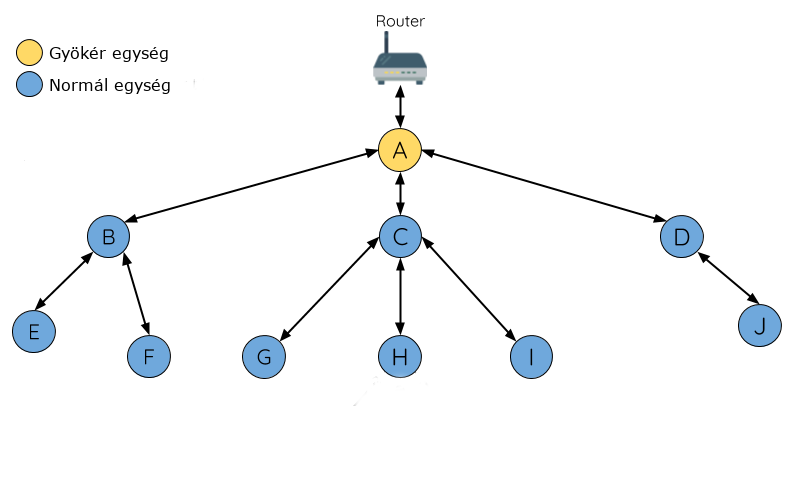
\includegraphics[width=150mm, keepaspectratio]{figures/mesh.png}
    \caption{A hálózat felépítése \cite{ESPMESH—29:online} }
    \label{fig:mesh_network}
\end{figure}


\subsubsection{Gyökér csomópont}
A hálózat felépítése ezek segítségével kezdődik. Ilyen egység akkor keletkezik, ha az adott csomópont többszöri REQUEST\_PARENT üzenet küldése után sem kap választ. Ebben az esetben kinevezi magát kezdő csomópontnak és beállítja szülő flag-et, ezzel is jelezve, hogy hozzá már lehet kapcsolódni. Ezeknek a csomópontoknak olyan további különleges tulajdonságuk is van, hogy ők tudnak kommunikálni a külvilággal, feltéve ha a konfigurációs fájlban engedélyezve van az MQTT használata. Az ide beérkező STATUS üzeneteket átalakítják MQTT-ben használt topikokká majd ezeket publikálják. Az általuk publikát topikokra fel is vannak iratkozva, ezért módosítás esetén ők alakítják vissza a Broker-től érkező infromációkat UPDATE üzenetekké majd továbbítják hálózatukon.

\subsubsection{Normál csomópont}
A normál csomópont akkor keletkezik, ha egy egység sikeresen rákapcsolódik egy a gyökér vagy egy másik csomópontra, ami szülőként is funkciónal. Sikeres kapcsolódás után engedélyezheti, hogy ő rá is lehessen kapcsolódni.



A hálózat felépítése során fontos, hogy egy csomópontra csak akkor lehessen csatlakozni, ha már ő is csatlakoztatva van valakihez ( kivétel a gyökér egység ). Ellenkező esetben létre jöhet olyan hálozat, ami nem tud a külvilággal kommunikálni. A másik fontos tulajdonság, hogy egy egységnek csak egy szülője lehet, hogy ne alaklujanak ki hurkok, ahol az üzenetek végtelenségig keringenének. Az utóbbi esetet egyébként egy plusz TTL paraméter bevezetésével kilehetne küszöbölni. A feltételek betartása esetében a hálózatnak végül egy fa struktúrája lesz.

Az egységek meghibásodásának detektálása időtúllépéssel segítségével történik. Minden egység tárol a hozzá kapcsolódott eszközökhöz egy időtúllépési számlálót, amiknek az értékeit periódikusan növeli. STATUS üzenet érkezése esetén az adott számlálót 0-ra állítja. A számlaló ha elér egy megadott értéket, akkor törli az egységet a táblájából. Az olyan esetekben, amikor a törölt egység megegyezik a szülő egységgel, akkor ismét elkezdi a szülő keresési lépést.

\subsection{Titkosítás}
Az egységek kommunikációjának titkosítására nem a beépített AES alapú algoritmus lett haszálva, hanem a felhasznált technológiáknál említett ChaCha szimmetrikus kulcsú rejtjelező. A jelenlegi verzióban a kulcsok nem kerülnek átküldésre a hálózaton, hanem az egységek flashmemóriájába vannak eltárolva egy konfig fájl részeként. Az eltárolt konfig fájlt a rendszer induláskor tölti be SPIFFS használatával és ez alapján inicializálja a változókat.
A rendszer a kiküldendő üzenet adatcsomagját titkosítja és ez kerül továbbításra a hálózatra. A eszközök az üzenet feldolgozását a tikosítás feloldásával kezdik és azután tudnak további döntést hozni, hogy nekik jött-e az üzenet vagy továbbítani szükséges. Utóbbi esetben újracsomagolás helyett, a memóriában lévő beérkező titkosított üzenetet továbbítja.
